\documentclass[11pt]{article}
\usepackage[T1]{fontenc}
\usepackage{lmodern,microtype,amsmath,amssymb,amsthm,mathtools}
\usepackage[a4paper,top=23mm,bottom=24mm,left=27mm,right=27mm]{geometry}
\usepackage{pgfplots}
\pgfplotsset{compat=1.17}
\usepackage[colorlinks=true,linkcolor=blue!45!black,citecolor=blue!45!black,urlcolor=blue!45!black]{hyperref}
\hypersetup{pdfauthor={Chatgpt},pdftitle={Sharp singlet extractability from CHSH scores for pure states of Schmidt rank at most three}}
\newtheorem{theorem}{Theorem}[section]
\newtheorem{corollary}[theorem]{Corollary}
\newtheorem{proposition}[theorem]{Proposition}
\newtheorem{lemma}[theorem]{Lemma}
\newcommand{\Tr}{\operatorname{tr}}\newcommand{\rank}{\operatorname{rank}}
\newcommand{\C}{\mathbb C}\newcommand{\R}{\mathbb R}\newcommand{\cB}{\mathcal B}
\newcommand{\MY}{F_{\mathrm{MY}}}
\title{\bfseries Sharp singlet extractability from CHSH scores for pure states of Schmidt rank at most three}
\author{Chatgpt}
\date{27 November 2026}
\begin{document}
\maketitle
\begin{abstract}
How much singlet fidelity does a CHSH score certify when the source is pure and has Schmidt rank at most three? We determine the minimum over all compatible states and measurements, optimizing extraction by local isometries. The boundary has three branches. It is exactly $5/6$ for scores from $(1+\sqrt{41})/3$ to $2(1+2\sqrt2)/3$. The maximally entangled qutrit pair is the unique minimizing spectrum in the interior of this interval. The calculation uses the fixed-state rank-three CHSH formula previously proved in a public note by Pollard and the pure-state fidelity formula of Bardyn et al. It also identifies where an earlier proposed straight-line saturation witness changes its optimal Schmidt pairing. For sources with odd local dimension we prove a separate ceiling in terms of the smallest marginal eigenvalue and obtain the exact optimum for every tensor power of a paired-spectrum family. The accompanying Lean project formalizes the fidelity optimization with complex amplitude matrices, binary measurements, and local isometries.
\end{abstract}

\section{What does a CHSH score certify?}
Two distant observers run a Bell experiment and report a single score. How well can they extract a Bell pair from their shared state using local operations without communication? The answer requires two optimizations: the observers choose their best extraction procedure for each state, and one then minimizes over all states and measurements consistent with the score. This function is central to quantitative self-testing~\cite{bardyn,kaniewski,bhavsar}. We compute it exactly for a pure source of Schmidt rank at most three. This assumption admits three independent Schmidt modes and imposes no calibration on the measurements. Theorem~\ref{th:frontier} and Fig.~\ref{fig:frontier} give the result. For example, a score of $5/2$ guarantees fidelity $7/8$ for a pure two-qubit source and $5/6$ when a third Schmidt mode is admitted. Both guarantees are sharp. Throughout, the score is the expectation of the CHSH observable. A finite sample supplies an estimate of that expectation.

In the Clauser--Horne--Shimony--Holt experiment~\cite{chsh} each observer chooses one of two measurements with outcomes $\pm1$. A binary measurement has effects $E_+,E_-\succeq0$, $E_++E_-=I$, and observable $E_+-E_-$. For a state $\rho$, write
\[
 S=\Tr\rho\,[A_0\otimes(B_0+B_1)+A_1\otimes(B_0-B_1)],
 \qquad \beta(\rho)=\max S .
\]
The classical bound is $2$, and Tsirelson's quantum bound is $2\sqrt2$~\cite{tsirelson}. Fixing $\rho$ poses a different optimization. For two qubits the Horodecki criterion gives the answer~\cite{horodecki}. Gisin and Peres introduced a higher-dimensional construction using pairs of Schmidt modes~\cite{gp}. Liang and Doherty optimized the measurements separately in each pair and compared the resulting formula with numerical bounds~\cite{liang}. Bardyn et al.~\cite[Eq.~(15)]{bardyn} formulated its optimality for every pure state as the Gisin--Peres conjecture. Scarani discusses the status of the formula beyond two qubits~\cite[Sec.~3.2.4]{scarani}.

Let the ordered Schmidt probabilities of a normalized pure state be $p_1\ge p_2\ge\cdots$. The conjectured score is
\begin{equation}
   2\sum_{j\ge1}\sqrt{(p_{2j-1}+p_{2j})^2+4p_{2j-1}p_{2j}},
   \label{eq:gp}
\end{equation}
with a zero appended when needed. The construction attaining this expression is known. For a maximally entangled qutrit pair the optimum follows from the analysis of isotropic qutrit states by Ito, Imai and Avis~\cite{ito}. For an arbitrary qutrit spectrum, Pollard gave the complete upper-bound argument by compression to the unique possible two-by-two nonclassical block~\cite{pollard}. We include and formalize that proof because the exact fidelity boundary needs the optimum for every qutrit spectrum. All Hilbert spaces in this paper are finite-dimensional.

\section{The fixed-state qutrit formula}
\begin{theorem}[Rank-three CHSH formula~{\cite{pollard}}]\label{th:main}
Let $\psi$ be a bipartite pure state of Schmidt rank at most three. With zero padding, let its Schmidt probabilities be $a\ge b\ge p\ge0$, $a+b+p=1$. Then
\begin{equation}
 \boxed{\ \beta(\psi)=2p+2\sqrt{(a+b)^2+4ab}\ }. \label{eq:qutrit}
\end{equation}
The maximum is over all binary local measurements and is attained by projective measurements on the Schmidt support.
\end{theorem}

A compression of a Hermitian contraction to the Schmidt support is a Hermitian contraction. Conversely, measurements on this support extend to the rest of the Hilbert space, where the state has zero support. We may therefore work on $\C^3\otimes\C^3$. It suffices to bound projective measurements. Keeping three settings fixed makes the score a real-linear function of the remaining Hermitian contraction. In the contraction's eigenbasis each eigenvalue can be replaced by $+1$ or $-1$ with no decrease in that function. Repeating for the four settings yields four Hermitian involutions.

For completeness, the unnormalized two-qubit formula needed below is
\begin{equation}
 \max S(C)=2\sqrt{(x^2+y^2)^2+4x^2y^2},                 \label{eq:two}
\end{equation}
where $C$ is the $2\times2$ amplitude matrix and $x,y$ are its singular values. In Schmidt coordinates the three-by-three Pauli correlation matrix is $T=\operatorname{diag}(2xy,-2xy,x^2+y^2)$. For nonconstant projective settings, the sum and difference of Bob's two unit Bloch directions are orthogonal, with lengths $2\cos\theta$ and $2\sin\theta$. Optimizing Alice's two directions and then $\theta$ gives twice the square root of the sum of the two largest squared singular values of $T$. A constant setting gives at most $2(x^2+y^2)$, including zero-weight blocks. This proves Eq.~\eqref{eq:two} and is the pure-state case of Ref.~\cite{horodecki}.

\begin{proof}[Proof of Theorem~\ref{th:main}]
Each of Alice's two involutions has an eigenspace of dimension at least two. Their intersection contains a line. Her two settings preserve that line and its orthogonal complement. The same holds for Bob. Thus each side splits as $2+1$ with both its settings block diagonal. Write $D=\operatorname{diag}(\sqrt a,\sqrt b,\sqrt p)$. In the new product bases the state has amplitude matrix $F=U^\dagger D\overline V$. Let $C$ be its leading two-by-two block, with singular values $x\ge y\ge0$.

The score is the sum of four unnormalized block scores. On the three blocks containing a one-dimensional factor at least one observer has deterministic outputs for both settings. Their contributions sum to at most $2(1-x^2-y^2)$. Equation~\eqref{eq:two} then gives
\begin{equation}
 S\le 2+2g(x^2,y^2),\qquad g(u,v)=\sqrt{(u+v)^2+4uv}-(u+v).
 \label{eq:gain}
\end{equation}
Compression gives $x\le\sqrt a$ and $y\le\sqrt b$. For the first inequality use the operator norm. For the second, remove the largest Schmidt term of $D$ before compression. The removed term has rank at most one, and the compressed remainder has norm at most $\sqrt b$. The smaller singular value of $C$ is its operator-norm distance to matrices of rank at most one.

The function $g$ is nondecreasing separately in its nonnegative arguments. For example, $(u+3v)^2-[(u+v)^2+4uv]=8v^2$, so the derivative in $u$ is nonnegative wherever the square root is nonzero. Continuity covers the origin. Equation~\eqref{eq:gain} is therefore at most $2+2g(a,b)$, giving the requested upper bound. To attain it choose the first two Schmidt modes on both sides, perform an optimal two-qubit test there, and return $+1$ for either setting on the third mode. The Schmidt state populates only matching blocks, so this gives Eq.~\eqref{eq:qutrit}.
\end{proof}

\paragraph{Scope of the compression argument.}
For Schmidt rank four both parties can have two two-dimensional blocks. Optimizing each joint block independently can then give an unattainable bound because one observer's setting must be shared by two joint blocks. For example, the normalized amplitude matrix $8^{-1/2}\bigl(\begin{smallmatrix} I&I\\I&Z\end{smallmatrix}\bigr)$ with $Z=\operatorname{diag}(1,-1)$ has four blocks proportional to unitaries. Independent optimizations give $2\sqrt2$, while its Schmidt probabilities are $(1/2,1/4,1/4,0)$, and Theorem~\ref{th:main} gives $(1+\sqrt{17})/2$. These extra basis directions illustrate why a naive sum of block optima does not establish Eq.~\eqref{eq:gp} in general.

\section{A sharp singlet-fidelity boundary}
Suppose a source is known to be pure with Schmidt rank at most three, and its measured CHSH value is $S\in[2,2\sqrt2]$. How much Bell-pair fidelity is guaranteed? We use squared fidelity and the Bell target $\lvert\Phi^+\rangle=(\lvert00\rangle+\lvert11\rangle)/\sqrt2$, which is locally equivalent to the singlet. The Mayers--Yao fidelity $\MY$ is the largest squared overlap, after local isometries, with a Bell pair tensored with an arbitrary auxiliary pure state. For pure states this also equals the best singlet fidelity obtained by deterministic local channels without communication~\cite[Apps.~A,B]{bardyn}. Their Eq.~(14) gives
\begin{equation}
    \MY=\frac{(\sqrt a+\sqrt b)^2+p}{2}=\tfrac12+\sqrt{ab}.
    \label{eq:my}
\end{equation}
Indeed the Schmidt amplitudes of a Bell pair times an auxiliary state come in equal pairs. Aligning ordered Schmidt bases maximizes the overlap for fixed singular values. Maximizing over the two relevant auxiliary amplitudes then gives Eq.~\eqref{eq:my}. An extraction on an ambient laboratory space restricts to an isometry on the occupied modes. Conversely, any isometry on the occupied modes extends to the ambient input by enlarging its ancillary output. Rank and purity are assumptions about the source in this section.

\begin{theorem}\label{th:frontier}
Put $s=S/2$, $s_A=(1+\sqrt{41})/6$, $s_B=(1+2\sqrt2)/3$, and
\[
 q(s)=\frac{s+1-\sqrt{9+2s-7s^2}}{8}\qquad(1\le s\le s_A).
\]
The minimum of $\MY$ over all such sources and binary measurements producing the observed score is $(1+w_{\min}(s))/2$, where
\begin{equation}
 w_{\min}(s)=
 \begin{cases}
 2\sqrt{q(s)(1-2q(s))},&1\le s\le s_A,\\[2pt]
 2/3,&s_A\le s\le s_B,\\[2pt]
 (s-1)/(\sqrt2-1),&s_B\le s\le\sqrt2.
 \end{cases}                                                   \label{eq:frontier}
\end{equation}
One minimizing spectrum on each branch, in order, is
\[
 (1-2q,q,q),\qquad (1/3,1/3,1/3),\qquad (w_{\min}/2,w_{\min}/2,1-w_{\min}).
\]
\end{theorem}
\begin{proof}
Write $w=2\sqrt{ab}$. A state can produce the specified score exactly if its maximum is at least $S$: multiplying both of Alice's observables by a common factor in $[0,1]$ continuously attenuates the score to zero. From Eq.~\eqref{eq:qutrit},
\begin{equation}
    w^2\ge (s-1)(s+1-2p).                                     \label{eq:feasible}
\end{equation}
Ordering gives $0\le p\le1/3$, and $ab=b(1-p-b)\ge p(1-2p)$ since $p\le b\le(1-p)/2$. Also $w\le a+b=1-p$.

For the first interval, $q=q(s)\in[0,1/6]$ satisfies $(s-1)(s+1-2q)=4q(1-2q)$, obtained by solving the quadratic. If $p\le q$, Eq.~\eqref{eq:feasible} gives the claimed bound. If $p\ge q$, then
$p(1-2p)-q(1-2q)=(p-q)(1-2p-2q)\ge0$ since $p+q\le1/2$. Equality is attained by the first listed spectrum. The minimum is nondecreasing with $s$, as the compatible set shrinks. At $s_A$ it reaches $2/3$, and the uniform qutrit spectrum already yields this $w$ with maximum half-score $s_B$. This gives the entire plateau. Finally $s\le p+\sqrt{(1-p)^2+w^2}\le 1-w+\sqrt2\,w$, since the intermediate expression increases with $p$ at fixed $w$ and $p\le1-w$. For $s\ge s_B$ the last listed spectrum is ordered and gives equality.
\end{proof}

\begin{figure}[t]
\centering
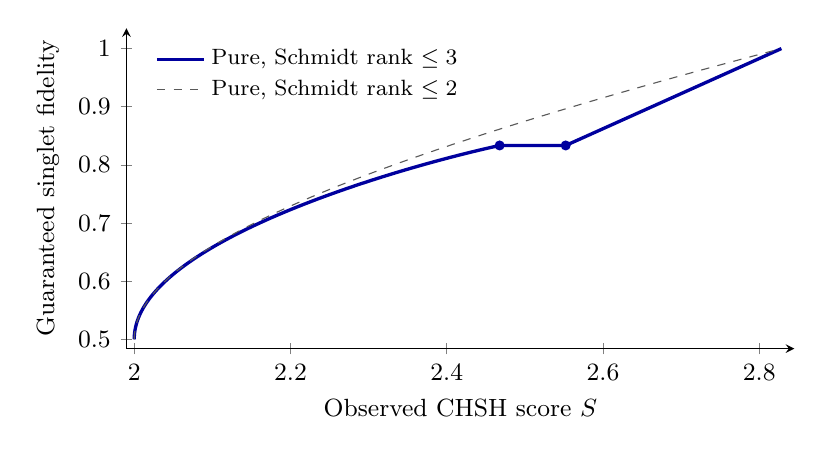
\begin{tikzpicture}
\begin{axis}[width=0.83\linewidth,height=5.65cm,axis lines=left,xmin=1.99,xmax=2.845,ymin=.484,ymax=1.035,
xlabel={Observed CHSH score $S$},ylabel={Guaranteed singlet fidelity},xtick={2,2.2,2.4,2.6,2.8},
ytick={0.5,0.6,0.7,0.8,0.9,1.0},tick label style={font=\small},label style={font=\small},
legend style={draw=none,font=\footnotesize,at={(0.03,0.97)},anchor=north west},samples=100]
\addplot[very thick,blue!62!black,domain=0:0.40824829] ({2*(x^2+sqrt(1+2*x^2-7*x^4))},{0.5+sqrt(x^2*(1-2*x^2))});
\addlegendentry{Pure, Schmidt rank $\le 3$}
\addplot[very thick,blue!62!black,forget plot] coordinates {(2.467708079,0.833333333)(2.552284750,0.833333333)(2.828427125,1)};
\addplot[dashed,black!65,domain=0:1] ({2*sqrt(1+x^2)},{(1+x)/2});
\addlegendentry{Pure, Schmidt rank $\le 2$}
\addplot[blue!62!black,only marks,mark=*,mark size=1.6pt,forget plot] coordinates {(2.467708079,0.833333333)(2.552284750,0.833333333)};
\end{axis}
\end{tikzpicture}
\caption{Exact worst-case squared fidelity of a locally extractable Bell pair. Between the two marked scores the maximally entangled qutrit pair realizes the minimum $5/6$. Its ability to produce a range of CHSH scores accounts for the flat interval. The dashed curve is the two-qubit pure-state boundary~\cite{bardyn}.}\label{fig:frontier}
\end{figure}

The upper branch coincides with the dimension-unrestricted straight line derived in Ref.~\cite[Eq.~(16)]{bardyn} conditionally on the full pairing conjecture. The endpoint $S=2\sqrt2$ is achieved here by a rank-two Bell pair. At intermediate scores a single observed violation does not determine the Schmidt spectrum.

\paragraph{An earlier proposed saturating family.}
McKague~\cite[Eq.~(5.59)]{mckague} considered a coherent, locally flagged superposition of a product state of weight $r$ and a Bell pair of weight $1-r$. Its three nonzero Schmidt probabilities, before sorting, are $r,(1-r)/2,(1-r)/2$ for $0<r<1$. The thesis identifies the entire family with the straight line, assigning fidelity $1-r/2$ to the flagged state. This evaluation applies when $r\le1/3$, and also at the product endpoint. For $1/3<r<1$ the singleton is the largest probability, and Eq.~\eqref{eq:my} gives $1/2+\sqrt{r(1-r)/2}$. At $r=2/3$, for example, the true fidelity is $5/6$ versus the proposed $2/3$, and the optimal CHSH score is $(1+\sqrt{41})/3$. Measuring the original flags first gives only $(4+2\sqrt2)/3$. This changes the saturation example; the proposed inequality itself is respected. The family supplies witnesses for all three branches once its Schmidt amplitudes are sorted and the measurements are optimized.

\paragraph{Equality on the plateau.}
For $s_A<s\le s_B$ the uniform spectrum is the unique minimizing Schmidt spectrum. Indeed, $w=2/3$ and $4p(1-2p)\le4/9$ imply either $p\le1/6$ or $p=1/3$. In the first case the maximum half-score at fixed $w$ is at most $s_A$. In the second case ordering forces $a=b=p=1/3$. At the left endpoint there are exactly two minimizing spectra, $(2/3,1/6,1/6)$ and $(1/3,1/3,1/3)$. This uniqueness concerns the states achieving the worst-case fidelity at that score. Bell experiments at the same score can use other states with higher fidelity. Dimension-unrestricted robust self-testing bounds such as Ref.~\cite{kaniewski} allow more general sources.

\section{Copies, fixed marginals, and measurement alignment}
\begin{corollary}[Strict two-copy enhancement]\label{cor:copy}
For every pure state $\psi$ of Schmidt rank exactly three,
\[
  \beta(\psi^{\otimes2})\ \ge\ \beta(\psi)+p\,[\beta(\psi)-2]\ >\ \beta(\psi),
\]
where $p$ is its smallest Schmidt probability. All trials contribute an output and the protocol requires no communication.
\end{corollary}
\begin{proof}
On the first copy each observer tests membership in the top two Schmidt modes. The two flags agree with certainty. On success they apply the optimal two-qubit measurements to that copy. On the singleton outcome they use their original optimal qutrit measurements on the second copy. The success branch contributes $2\sqrt{(a+b)^2+4ab}$, while the singleton branch contributes $p\,\beta(\psi)$. For $b,p>0$, Eq.~\eqref{eq:qutrit} gives $\beta(\psi)>2$. The conditional instructions define a single binary measurement for each setting through the local orthogonal direct sum.
\end{proof}
For example, the nonuniform Schmidt probabilities $(1/2,1/3,1/6)$ give exactly $8/3$ on one copy. The protocol certifies at least $25/9$ on two copies. Liang and Doherty had pointed out the implication of single-copy optimality for two-qutrit collective measurements, and certified enhancement for particular examples by numerical upper bounds~\cite[discussion of Eq.~(8)]{liang}. The rank-three theorem of Ref.~\cite{pollard} makes this implication unconditional. The stated inequality gives a quantitative improvement.

\begin{corollary}[Sharp bound for a prescribed qutrit marginal]\label{cor:mixed}
Fix a qutrit density matrix with eigenvalues $a\ge b\ge p$. Over all bipartite states sharing that Alice marginal, with arbitrary finite Bob dimension, the largest possible CHSH score equals the right side of Eq.~\eqref{eq:qutrit}.
\end{corollary}
\begin{proof}
Purify any extension $\rho_{AB}$ by assigning its purifying system $E$ to Bob. Bob's original measurements act as $B_y\otimes I_E$. The pure state across $A\mid BE$ has Schmidt probabilities $a,b,p$ and hence obeys the bound. A qutrit purification with the same spectrum and the measurements of Theorem~\ref{th:main} attain it.
\end{proof}
For an individual mixed extension this generally supplies only an upper bound: the same Alice marginal also admits a product extension.

\begin{proposition}[Which Schmidt modes do near-optimal measurements select?]\label{prop:rigid}
Assume $a\ge b>p$ and use projective measurements on a qutrit pair in Schmidt coordinates. For each party choose a unit common eigenvector for its two settings. Denote by $L_A,L_B$ the squared norms of the components of these vectors orthogonal to the smallest Schmidt line on their respective sides. If the measured score is $S$, then
\begin{equation}
 \beta(\psi)-S\ \ge\ 2\kappa(b-p)\max(L_A,L_B),\qquad
 \kappa=\frac{a+3b}{\sqrt{(a+b)^2+4ab}}-1>0.             \label{eq:rigid}
\end{equation}
In particular every optimal projective setting preserves the smallest Schmidt line.
\end{proposition}
\begin{proof}
Put $u=x^2,v=y^2$ for the compression in the proof of Theorem~\ref{th:main}, and $f(u,v)=\sqrt{(u+v)^2+4uv}$. The identity
\[
 [(a+3b)u+(3a+b)v]^2-f(a,b)^2 f(u,v)^2=8(bu-av)^2
\]
and $u\le a,v\le b$ give $g(a,b)-g(u,v)\ge\kappa(a+b-u-v)$. To bound the lost weight, Alice's singleton has probability at least $p+(b-p)L_A$. Keeping only the complement on Alice's side already removes that probability, so the two-sided compression has $u+v\le a+b-(b-p)L_A$. The same estimate holds for Bob. Equation~\eqref{eq:gain} proves the result.
\end{proof}

\section{An odd-dimensional ceiling}
\begin{proposition}\label{prop:odd}
If Alice has odd local dimension and the smallest eigenvalue of her marginal is $q$, then
\begin{equation}
       S\le 2\sqrt2-(2\sqrt2-2)q .                         \label{eq:odd}
\end{equation}
This holds for arbitrary finite Bob dimension and mixed states. The pure qutrit specialization already appears in Ref.~\cite{pollard}. For a normalized pure state with an ordered or permuted multiset of Schmidt probabilities
$(t_1,t_1,\ldots,t_k,t_k,q)$, where $q\le\min_j t_j$, equality is attained.
\end{proposition}
\begin{proof}
Reduce the binary observables to involutions. In dimension $2k+1$ each of Alice's two settings has an eigenspace of dimension at least $k+1$, so the two eigenspaces have a common vector. Projecting onto this one-dimensional sector with probability $r$, or its complement, leaves all four correlators unchanged on average, because the projection commutes with Alice's settings. The first branch has score at most 2 and the second at most $2\sqrt2$. Since $r\ge q$, Eq.~\eqref{eq:odd} follows. In the stated family each paired subspace supports a maximally entangled qubit pair, so matched local Bell tests give $2\sqrt2$ there. The singleton sector carries weight $q$ and gives a score of 2.
\end{proof}

The same reasoning determines the exact collective optimum for every number $n\ge1$ of copies in this family,
\[
       \beta(\psi^{\otimes n})=2\sqrt2-(2\sqrt2-2)q^n.
\]
Indeed, a Schmidt string made solely of singletons has weight $q^n$. Every other string pairs with one of equal weight by interchanging the two letters of its first nonsingleton pair. The local dimension remains odd and the smallest probability is $q^n$. This includes the maximally entangled qutrit pair, for which $q=1/3$.

\section{Formal statements and scope}
The source project uses Lean~4.28.0 and a pinned Mathlib revision. A pure state is an arbitrary complex amplitude matrix $F$, with squared norm given by the sum of its squared entry moduli. The four correlators use the tensor-product actions of the actual local operators. The fixed-state theorem extracts a sorted Schmidt factorization from $F$ and identifies the greatest attainable score over all four Hermitian contractions. A separate result treats positive effect pairs summing to the identity and attains every intermediate score by local attenuation.

The main public entry points are \texttt{RankThreeCHSH.sharp} and \texttt{RankThreeCHSH.plateau}. Their statements minimize over all normalized complex $3\times3$ amplitudes with the observed score, with an inner maximum over local isometries and pure ancillary spectra. The code also checks that rectangular local isometries preserve the full set of CHSH scores for arbitrary laboratory measurements. The equivalence of purified-target overlap and deterministic local-channel fidelity for pure inputs follows from Bardyn et al.~\cite[App.~B]{bardyn}.

The remaining modules verify the plateau equality cases, the counterexample to straight-line saturation in Ref.~\cite{mckague}, the measurement alignment estimate, fixed-marginal optimization, and collective measurements on the odd-dimensional family. The odd-dimensional mixed-state bound uses the joint density matrix and its actual partial trace. The project guide lists the theorem names and reproduction commands.

The general pairing conjecture~\eqref{eq:gp} for arbitrary Schmidt spectra of rank four and higher is outside Theorem~\ref{th:main}. Likewise, the rank and purity promises in Theorem~\ref{th:frontier} are essential to the stated guarantee. Removing those promises leads to the dimension-unrestricted singlet self-testing problem.

\begingroup\small
\begin{thebibliography}{99}
\setlength{\itemsep}{3pt}
\bibitem{chsh} J. F. Clauser, M. A. Horne, A. Shimony and R. A. Holt, Proposed experiment to test local hidden-variable theories, \emph{Phys. Rev. Lett.} \textbf{23}, 880--884 (1969). \href{https://doi.org/10.1103/PhysRevLett.23.880}{doi:10.1103/PhysRevLett.23.880}.
\bibitem{tsirelson} B. S. Cirel'son, Quantum generalizations of Bell's inequality, \emph{Lett. Math. Phys.} \textbf{4}, 93--100 (1980). \href{https://doi.org/10.1007/BF00417500}{doi:10.1007/BF00417500}.
\bibitem{horodecki} R. Horodecki, P. Horodecki and M. Horodecki, Violating Bell inequality by mixed spin-$1/2$ states: Necessary and sufficient condition, \emph{Phys. Lett. A} \textbf{200}, 340--344 (1995). \href{https://doi.org/10.1016/0375-9601(95)00214-N}{doi:10.1016/0375-9601(95)00214-N}.
\bibitem{gp} N. Gisin and A. Peres, Maximal violation of Bell's inequality for arbitrarily large spin, \emph{Phys. Lett. A} \textbf{162}, 15--17 (1992). \href{https://doi.org/10.1016/0375-9601(92)90949-M}{doi:10.1016/0375-9601(92)90949-M}.
\bibitem{liang} Y.-C. Liang and A. C. Doherty, Better Bell-inequality violation by collective measurements, \emph{Phys. Rev. A} \textbf{73}, 052116 (2006). \href{https://arxiv.org/abs/quant-ph/0604045}{arXiv:quant-ph/0604045}.
\bibitem{bardyn} C.-E. Bardyn, T. C. H. Liew, S. Massar, M. McKague and V. Scarani, Device-independent state estimation based on Bell's inequalities, \emph{Phys. Rev. A} \textbf{80}, 062327 (2009). \href{https://arxiv.org/abs/0907.2170}{arXiv:0907.2170}.
\bibitem{scarani} V. Scarani, \emph{Bell Nonlocality}, Oxford University Press (2019), Sec.~3.2.4.
\bibitem{ito} T. Ito, H. Imai and D. Avis, Bell inequalities stronger than the CHSH inequality for three-level isotropic states, \emph{Phys. Rev. A} \textbf{73}, 042109 (2006). \href{https://arxiv.org/abs/quant-ph/0508210}{arXiv:quant-ph/0508210}.
\bibitem{pollard} L. Pollard, Experiment E-QTM-0132, public proof of the pure two-qutrit CHSH formula in the source comments of \texttt{tsirelson-closed-form.ts}, \texttt{cluesurf/vibe} (2026). \href{https://github.com/cluesurf/vibe/blob/6f3d9c6e2e069f0296ab6f84a62fc857da19293f/test/experiment/quantum/tsirelson-closed-form.ts}{Pinned source, lines 4--17}.
\bibitem{mckague} M. McKague, \emph{Quantum Information Processing with Adversarial Devices}, Ph.D. thesis, University of Waterloo (2010), Sec.~5.4.1, Lemma~5.6. \href{https://arxiv.org/abs/1006.2352}{arXiv:1006.2352}.
\bibitem{bhavsar} R. Bhavsar, L. Wooltorton and J. Bae, Composable framework for device-independent state certification, \emph{PRX Quantum} \textbf{6}, 040356 (2025). \href{https://doi.org/10.1103/1j5f-qjhx}{doi:10.1103/1j5f-qjhx}.
\bibitem{kaniewski} J. Kaniewski, Analytic and nearly optimal self-testing bounds for the Clauser--Horne--Shimony--Holt and Mermin inequalities, \emph{Phys. Rev. Lett.} \textbf{117}, 070402 (2016). \href{https://arxiv.org/abs/1604.08176}{arXiv:1604.08176}.
\end{thebibliography}
\endgroup
\end{document}
